\documentclass[a4paper,12pt]{article}
\usepackage[utf8]{inputenc}%%seul package à charger : pour éviter les problèmes sordides d'encodage
\usepackage[fiche]{andre}%%bon eh bien sûr...
\usepackage{wrapfig}
\usepackage{subfigure}
%%fiche, psc pour faire une fiche
%%rapport, psc pour faire un rapport
%%pour insérer du code : \langage{java} , puis \begin{lstlisting} \end{lstlisting}
%%pour insérer des guillemets : \eg \og

\title{Synthétiseur automatique de documents\\ PSC X2013}

\renewcommand{\petittitre}{PSC INF02}
\author{Fernandes-Pinto-Fachada Sarah, Schrottenloher Andr\'e, Angibault Antonin,\\
Hufschmitt Th\'eophane, Cao Zhixing, Boisseau Guillaume}

\date{24 avril 2015}

\fancypagestyle{temp}{
  \fancyhead[L]{}
  \fancyhead[R]{}

  \fancyfoot[R]{\raisebox{0.3cm} PSC X2013 - INF02}
\fancyfoot[L]{
\includegraphics[height=1cm]{logohori}}
\fancyfoot[C]{}
}


\begin{document}

%\titrelong%%une page complète
\titrecourt %titre plus court, typiquement pour les fiches
%\thispagestyle{temp}

%\subsection*{Résumé}

Notre projet a pour ambition \textbf{d'analyser sémantiquement un texte}, de manière automatique, afin de produire un \textbf{résumé synthétique} de celui-ci. \\


Les méthodes actuelles de résumé automatique se tournent en grande partie vers les outils statistiques : fréquences d'apparition de mots, sélection de mots-clés. Sans pour autant nous départir de la manipulation de grandes quantités de données textuelles, nous essayons d'introduire un véritable facteur de \textbf{compréhension du texte}, en manipulant des informations sémantiques ; qui sont porteuses d'un véritable sens. 

\begin{figure}
 \begin{minipage}[b]{.46\linewidth}
  \centering
  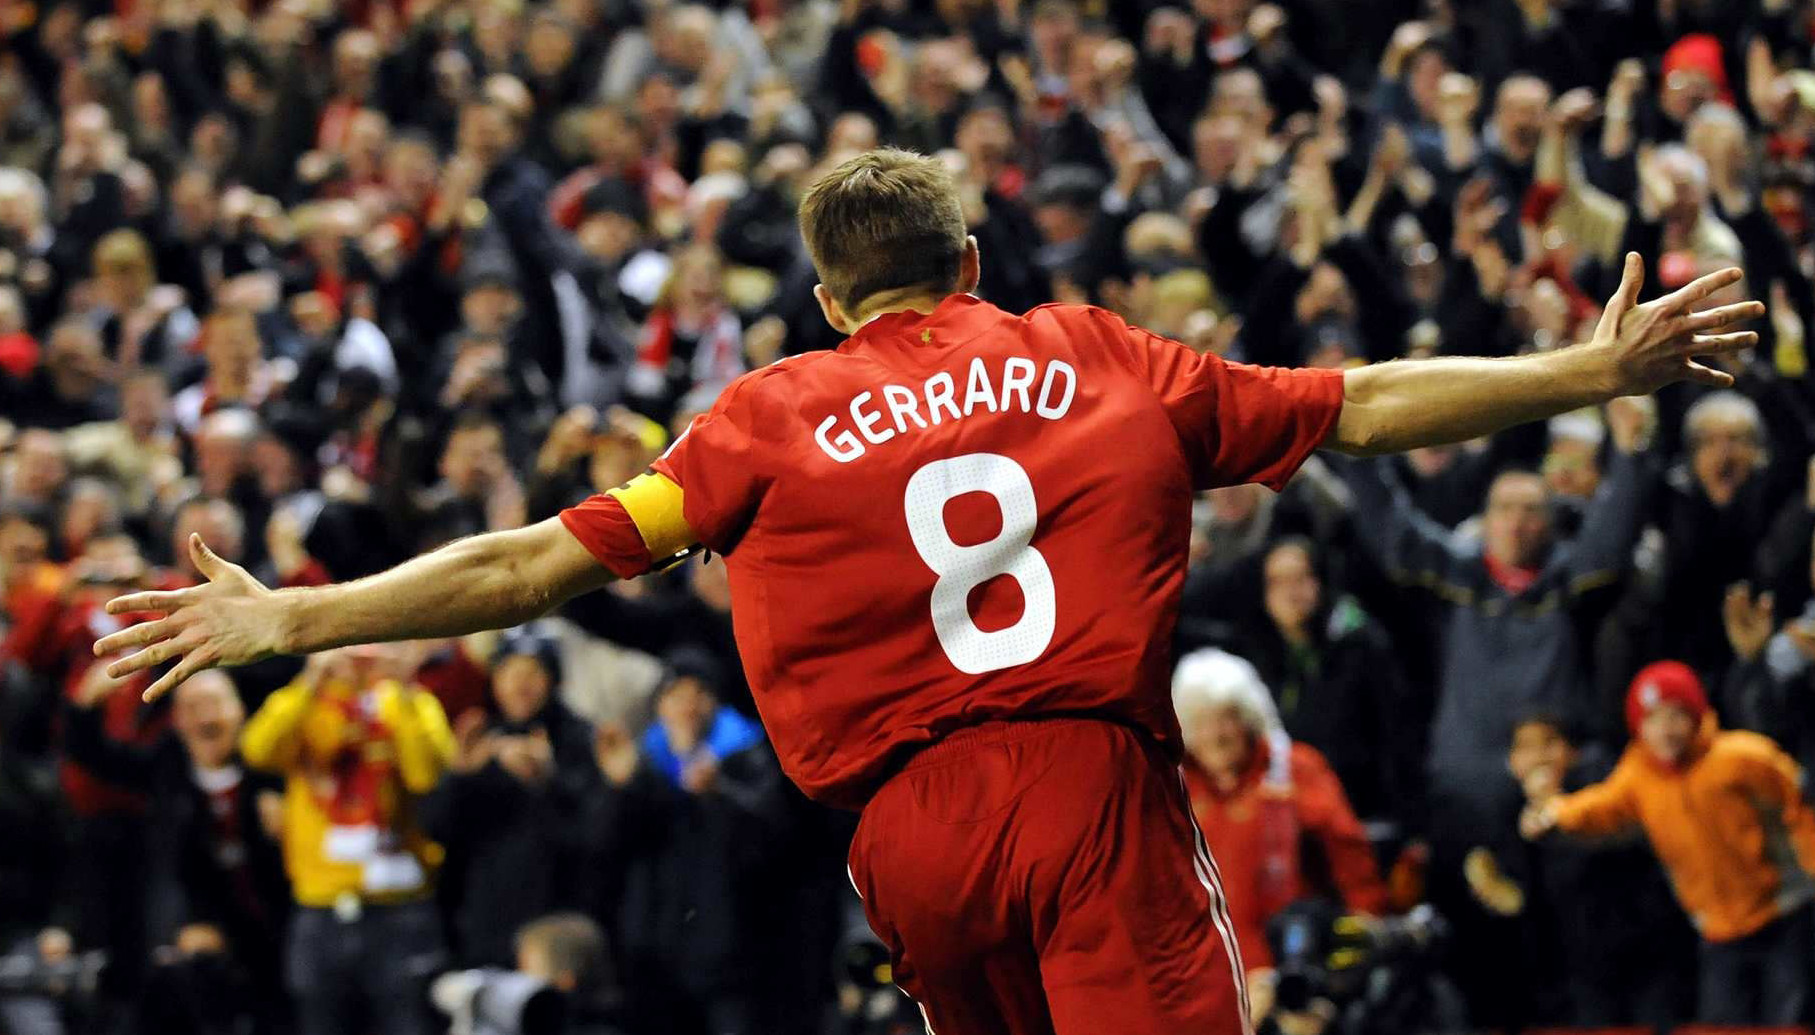
\includegraphics[width=7cm]{./gerrard.jpg}
  \caption{premiere figure \label{fig1}}
 \end{minipage} \hfill
 \begin{minipage}[b]{.46\linewidth}
  \centering
  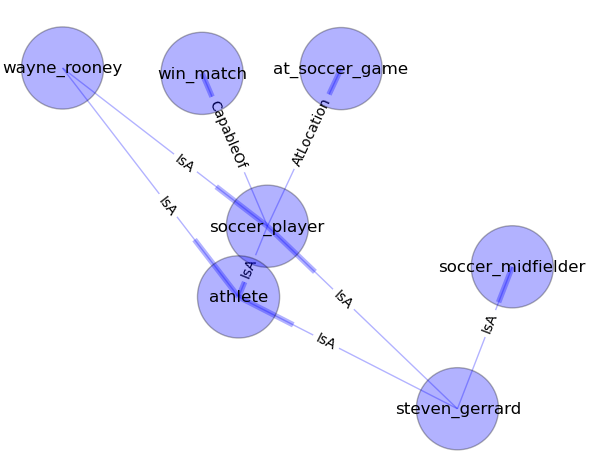
\includegraphics[width=9cm]{./figure_1.png}
  \caption{deuxieme figure \label{fig2}}
 \end{minipage}
\end{figure}


\begin{figure}[ht]
\begin{center}
  \subfigure[I]{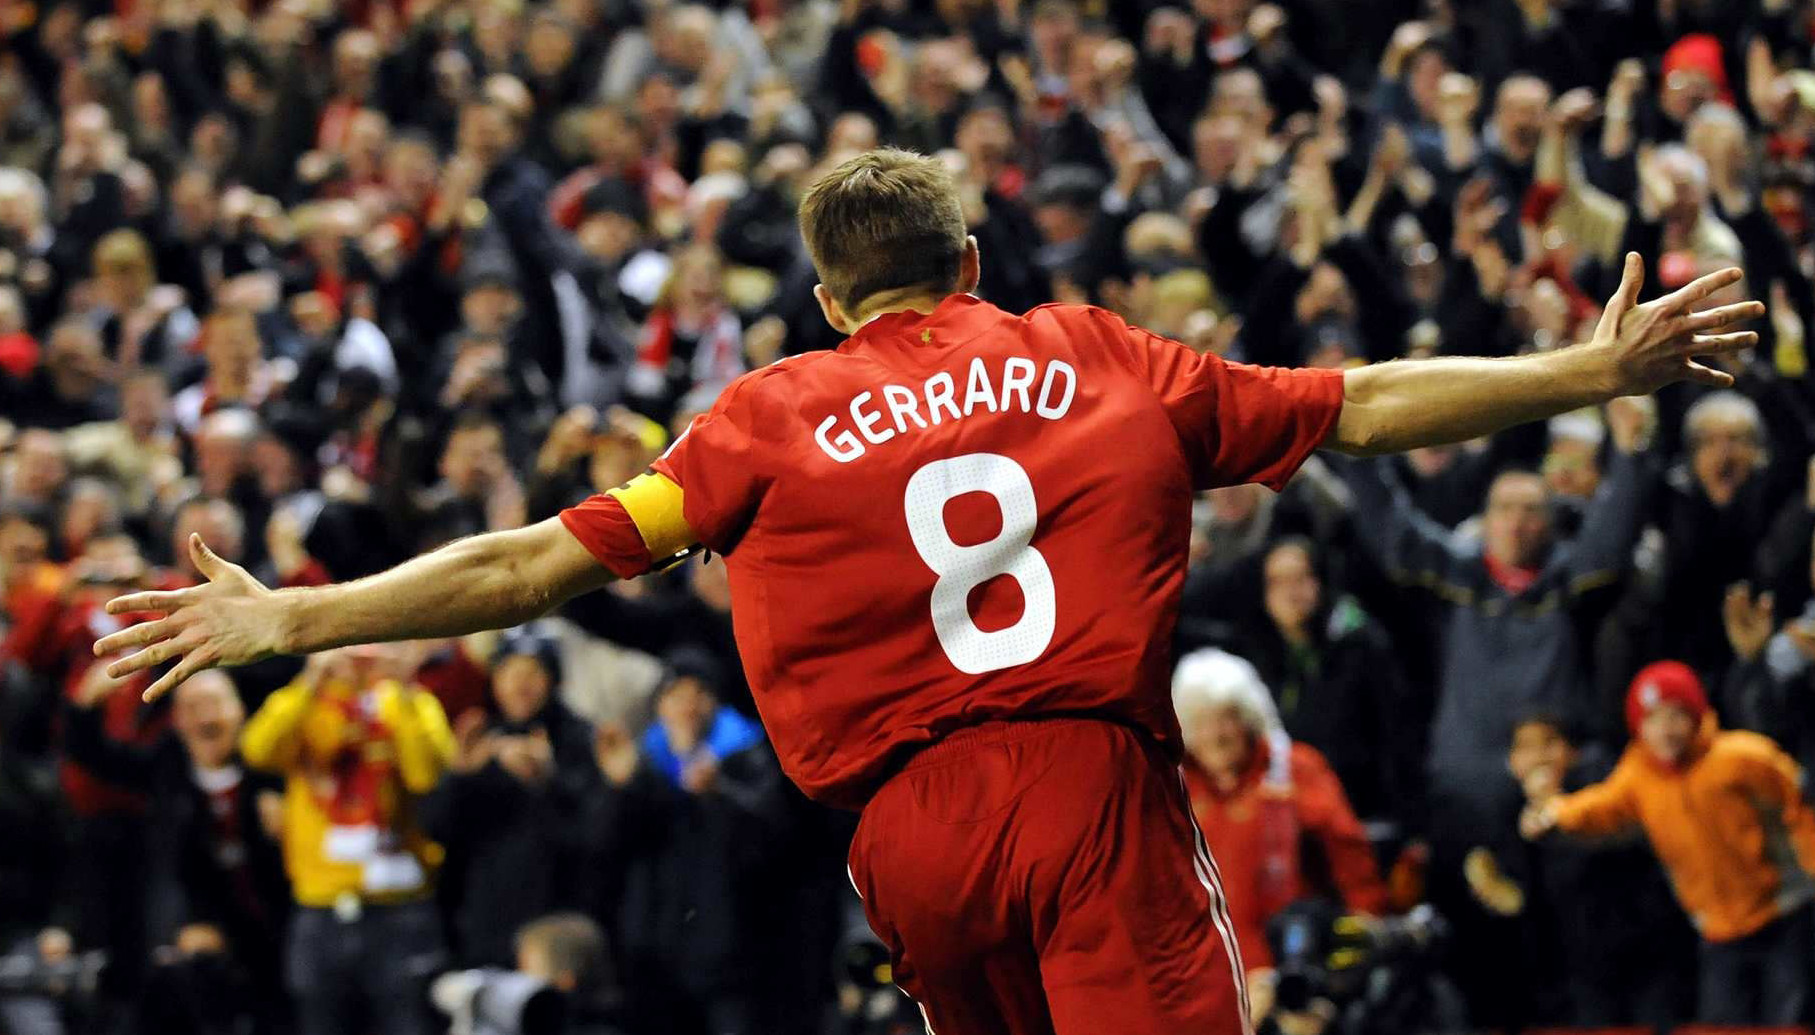
\includegraphics[width=7cm]{./gerrard.jpg}}\quad
  \subfigure[II]{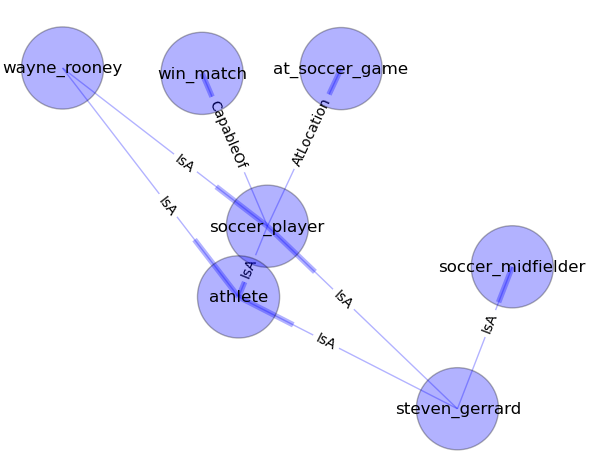
\includegraphics[width=9cm]{./figure_1.png}}\\
\end{center}
\caption{Des données brutes à la représentation des connaissances}
\label{fig:inf}
\end{figure}

\begin{figure}[!h]
  \centering 
  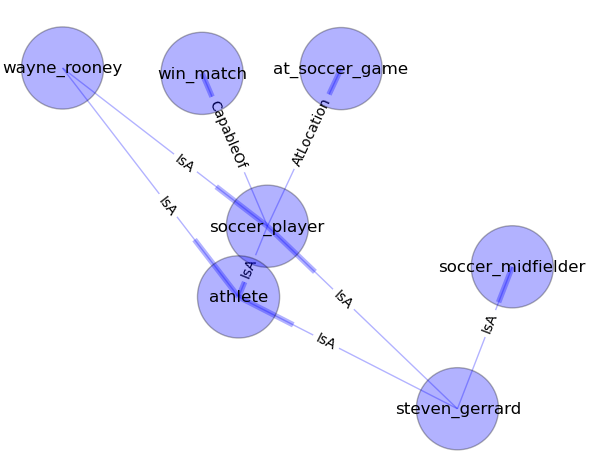
\includegraphics[width=10cm]{./figure_1.png}
\end{figure}


Ce point de vue original nous a amenés à explorer différents sous-problèmes, de l'analyse syntaxique à la représentation de données sémantiques en passant par l'introduction de structures de données malléables, dans le but d'y reconstruire l'information du texte et d'y sélectionner les informations pertinentes recherchées (nous nous sommes concentrés sur l'analyse d'articles de sport).


\begin{wrapfigure}{r}{6cm}
  \centering 
  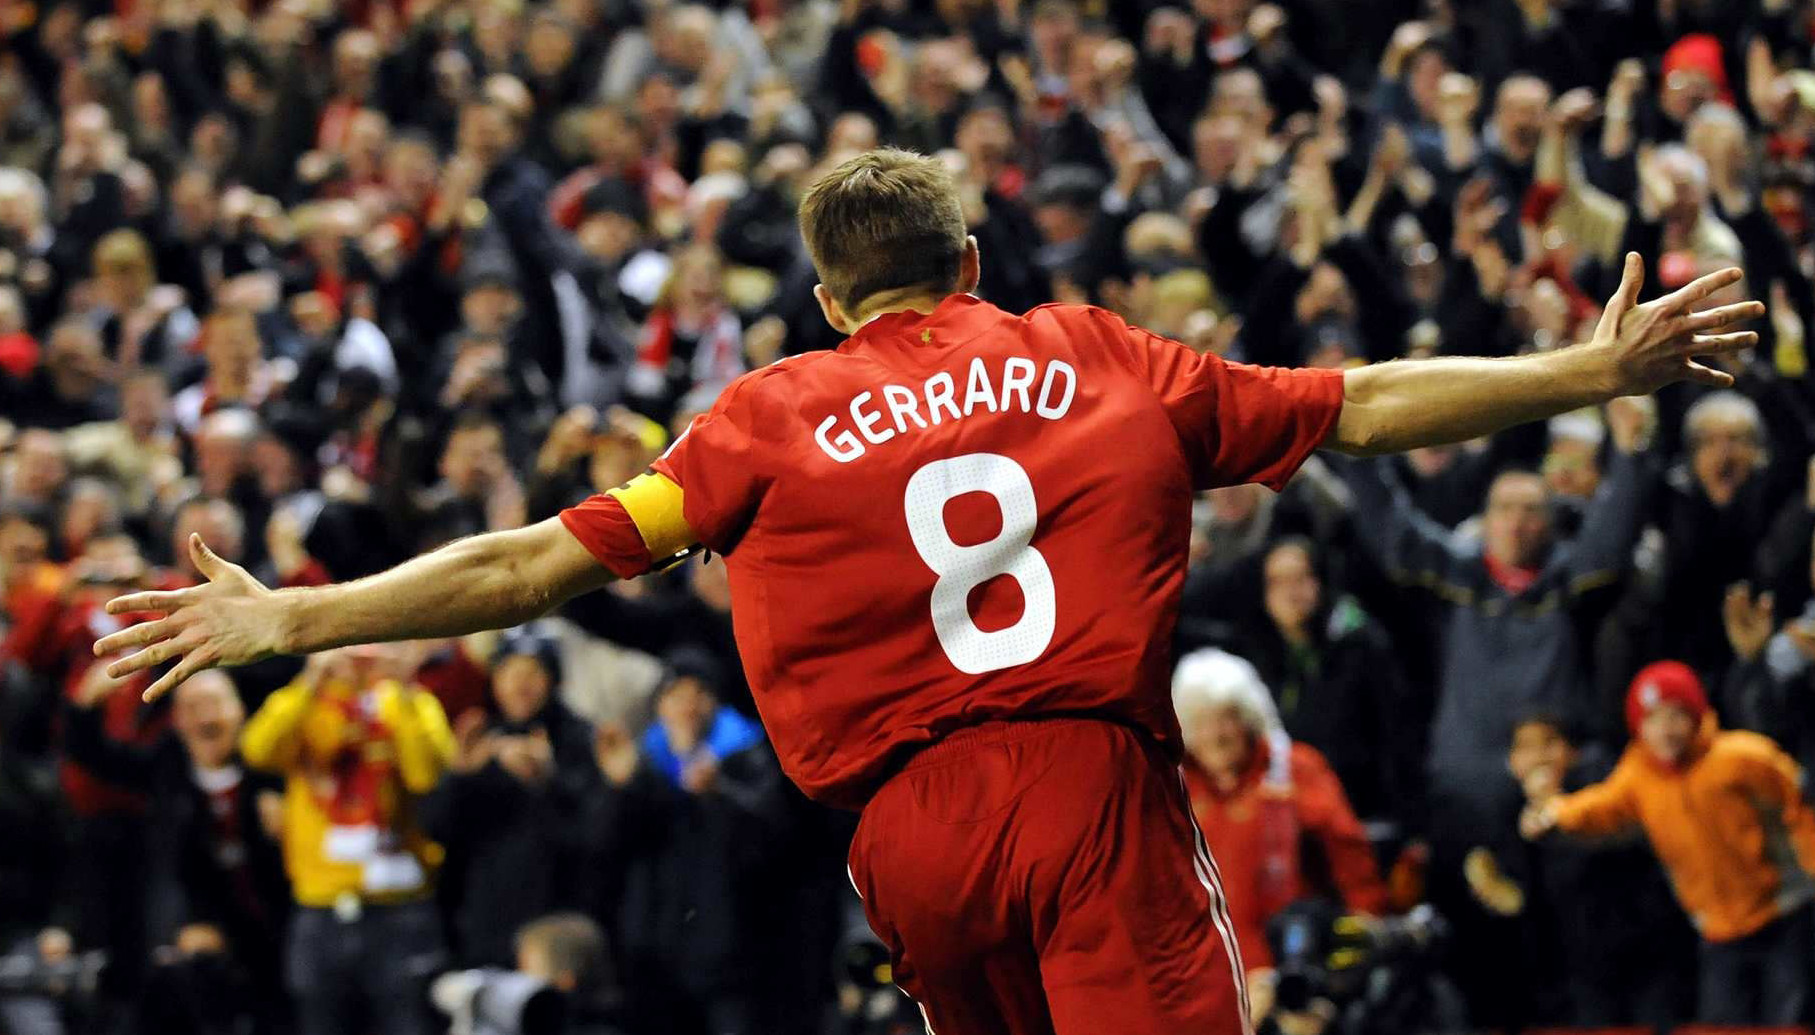
\includegraphics[width=6cm]{./gerrard.jpg}
\end{wrapfigure}

\subsection*{Contacts}

\begin{itemize}
 \item \textbf{Antonin Angibault} (chef de projet)~: \href{mailto:antonin.angibault@polytechnique.edu}{antonin.angibault@polytechnique.edu} ;
 \item \textbf{Théophane Hufschmitt}~: \href{mailto:theophane.hufschmitt@polytechnique.edu}{theophane.hufschmitt@polytechnique.edu}.
\end{itemize}

 
\end{document}



